\documentclass[russian,utf8,nocolumnxxxi,nocolumnxxxii]{eskdtext}
\usepackage[T1,T2A]{fontenc}
\usepackage[utf8]{inputenc}
\usepackage{amssymb,amsmath}
\usepackage{tikz}
\usepackage{siunitx}
\usepackage[american,cuteinductors,smartlabels]{circuitikz}
\usepackage[backend=biber]{biblatex}
\addbibresource{error_estimation_otchet.bib}
\usepackage[]{hyperref}
\hypersetup{
colorlinks=true,
}

\usepackage{textcomp}
\newcommand{\No}{\textnumero}
%Титульный лист
\ESKDdepartment{Федеральное агенство по образованию}

\ESKDcompany{Санкт-Петербургский государственный электротехнический университет ЛЭТИ}

\ESKDtitle{Пояснительная записка к курсовой работе}
\ESKDsignature{Вариант 3}
\ESKDauthor{Домнин А.В.}
\ESKDchecker{Прокшин А.Н.}
\ESKDdocName{по дисциплине "Информатика"}
\begin{document}
\maketitle
% 1 лист работы

\tableofcontents


\newpage

\section{Цель курсовой работы}
Уметь применять персональный компьютер и математические пакеты прикладных программ в инженерной деятельности.
\clearpage
\newpage
\section{Решение уравнения и исследование функции}
\subsection{Решение уравнения вида} f(x) = g(x)
\begin{equation}
f(x)= \sqrt{3\mathstrut}sin(x) + cos(x)
\end{equation}
\begin{equation}
g(x)=cos\left(2x+\frac n{3} \right)+1
\end{equation}
Пользуясь математическим пакетом SMath были получены следующие корни уравнения на интервале от 0 до 5п/6\\
\begin{equation}
x=2.618
\end{equation}
\subsection {Исследование функции}
На рисунке 1 изображена функция на интервале от -7 до 7\\ 
Область определения функции- функция определена на всем промежутке от (-{$\infty;+\infty$})
\begin{figure}[!ht]
    \centering
\begin{tikzpicture}[yscale=1,xscale=1]
%Построение осей
\draw[thin,->](-7,0)--(7,0) node [right] {$X$};
\draw[thin,->](0,-2)--(0,5) node [left] {$Y$};
%Построение графика
\draw [domain=-7:7, help lines,thick,smooth, red] plot ({\x},{sqrt(3)*sin(\x r)+cos(\x r)-cos((2*\x r)+(pi/3 r))+1});
%подпись 0
\node [below] {$0$};
\draw (5,6)node [black]{$\sqrt{3\mathstrut}\cdot sin(x)+cos(x)-cos\left(2x+\frac n{3}\right)+1$};
\end{tikzpicture} 
    \caption{Построение графика функции}
    \label{fig:my_label}
\end{figure}

Согласно задания функция должна быть определена на участке от 0 до 5п/6, на рисунке 2 изображен график функции
\begin{figure}[!ht]
    \centering
\begin{tikzpicture}[yscale=2.5,xscale=2.5]
%Построение осей
\draw[thin,->](0,0)--(3,0) node [right] {$X$};
\draw[thin,->](0,-0.2)--(0,5) node [left] {$Y$};
%Построение графика на участке от 0 до 5п/6
\draw [domain=0:2.616, help lines,thick,smooth, red] plot ({\x},{sqrt(3)*sin(\x r)+cos(\x r)-cos((2*\x r)+(pi/3 r))+1});
\node [below] {$0$};
%Построение перпендикуляра,точки максимума
\draw[thin,black,dashed] (2.618,0.5)--(2.618,0) node [below] {$2.618$};
\draw (1.05,0) node [below] {$1.05$};%точка максимума по Х
\draw (0,4) node [left] {$4$};%точка максимума по У
\draw[thin,black,dashed] (1.05,0)--(1.05,4);%построение вертикали
\draw[thin,black,dashed] (0,4)--(1.05,4);%построение горизонтали
\end{tikzpicture}
\caption{Построение графика функции на ограниченном участке}
    \label{fig:my_label}
\end{figure}
Корни уравнения вида представлены ниже
\begin{equation}
\sqrt{3\mathstrut}\cdot sin(x)+cos(x)-cos\left(2x+\frac n{3}\right)+1
\end{equation}
\begin{equation}
x=2.618
\end{equation}
На участке от 0 до 5п/6 функция имеет один "0" и он находится в точке 2,618 иллюстрирует график. Максимум находится в точке x=1.05, y=4. Функция является периодической, и является нечетной, так как меняет знак.
\begin{equation}
\sqrt{3\mathstrut}\cdot sin(-x)+cos(-x)-cos\left((-2x)+\frac n{3}\right)+1
\end{equation}
\begin{equation}
-\sqrt{3\mathstrut}\cdot sin(x)+cos(x)-cos\left(2x+\frac n{3}\right)+1
\end{equation}
Нули функции,то есть точка пересечения с осями координат: х=0,y=1.5.
Первая производная функции равна и определяется через пакет Reduce Algebra
\begin{equation}
\sqrt3cos(x)+2sin\left(\frac{n+6x}{3}\right)-sin(x)
\end{equation}
График производной приведен на рисунке 3 % 1 производная
\begin{figure}[!ht]
    \centering
\begin{tikzpicture}[yscale=1,xscale=1]
%Построение осей
\draw[thin,->](-5,0)--(5,0) node [right] {$X$};
\draw[thin,->](0,-5)--(0,5) node [left] {$Y$};
%Построение графика производной на всем участке 
\draw [domain=-7:7, help lines,thick,smooth, red] plot ({\x},{sqrt(3)*cos(\x r)+2*sin((pi r+6*\x r)/3)-sin(\x r)});
\node [below] {$0$};
\end{tikzpicture}
\caption{Построение графика производной}
\label{fig:my_label}
\end{figure}
%Построение графика производной на участке от 0 до 5п/6
\begin{figure}[!ht]
    \centering
\begin{tikzpicture}[yscale=1,xscale=1]
%Построение осей
\draw[thin,->](0,0)--(2.9,0) node [right] {$X$};
\draw[thin,->](0,0)--(0,5) node [left] {$Y$};
%производная на участке
\draw [domain=0:2.618, help lines,thick,smooth, red] plot (({\x},{sqrt(3)*cos(\x r)+2*sin((pi r+6*\x r)/3)-sin(\x r)});
\node [left] {$0$};
%Построение перпендикуляра,точек максимума и минимума
\draw[thin,black,dashed] (0,3.52)--(0.11,3.52) node [left] {$3.52$};%точка максимума по У
\draw[thin,black,dashed] (0.11,3.52)--(0.11,0) node [right,below] {$0.11$};%точка максимума по Х
\draw (1.05,0) node [right,above] {$1.05$};%ноль
\draw[thin,black,dashed] (1.98,0)--(1.98,-3.52);%минимум по У
\draw (1.98,0) node [right,below] {$1.98$};
\draw (1.98,-3.52) node [right,below] {$-3.52$};
\end{tikzpicture}
\caption{Построение графика производной на ограниченном участке}
    \label{fig:my_label}
\end{figure}
%Критические точки
Критические точки функции при которых производная функции равна 0
\begin{equation}
\sqrt3cos(x)+2sin\left(\frac{n+6x}{3}\right)-sin(x)=0
\end{equation}
Откуда корни уравнения равны на ограниченном участке,находятся через математический пакет Smath

\begin{equation}
x=1.047
\end{equation}

Для определения поведения функции на интервале от (0;1.047) необходимо определить производную.
Производная принимает положительное значение,следовательно она возрастает
Например в "0".
На участке (1,047;5n/6) принимает отрицательные значения, следовательно она убывает.\\
Для определения выпуклости и вогнутости и точек перегиба необходимо найти вторую производную.Для нахождения был применен пакет Reduce Algebra
\begin{equation}
4\cdot\cos\left(\frac{n+6x}{3}\right)-cos(x)-\sqrt3\cdot\sin(x)
\end{equation}

Для отыскания точек перегиба необходимо решить уравнение вида на промежутке
\begin{equation}
4\cdot\cos\left(\frac{n+6x}{3}\right)-cos(x)-\sqrt3\cdot\sin(x)=0
\end{equation}

Корни которого представлены ниже
\begin{equation}
x_1=0.1113,x_2=1.9831
\end{equation}
Откуда точки определятся при подстановке корней в уравнение.
\begin{equation}
y_1=-0.0003,y_2=-0.0002
\end{equation}
Функция выпукла на промежутке 0 до 0.1113, так как вторая производная принимает значение больше
Функция вогнута на промежутке 0.1113 до 1.9831  так как вторая производная принимает значение меньше
График второй производной функции вида
\begin{equation}
4\cdot\cos\left(\frac{n+6x}{3}\right)-cos(x)-\sqrt3\cdot\sin(x)
\end{equation}
представлен ниже,на рисунке 5
\begin{figure}[!ht]
    \centering
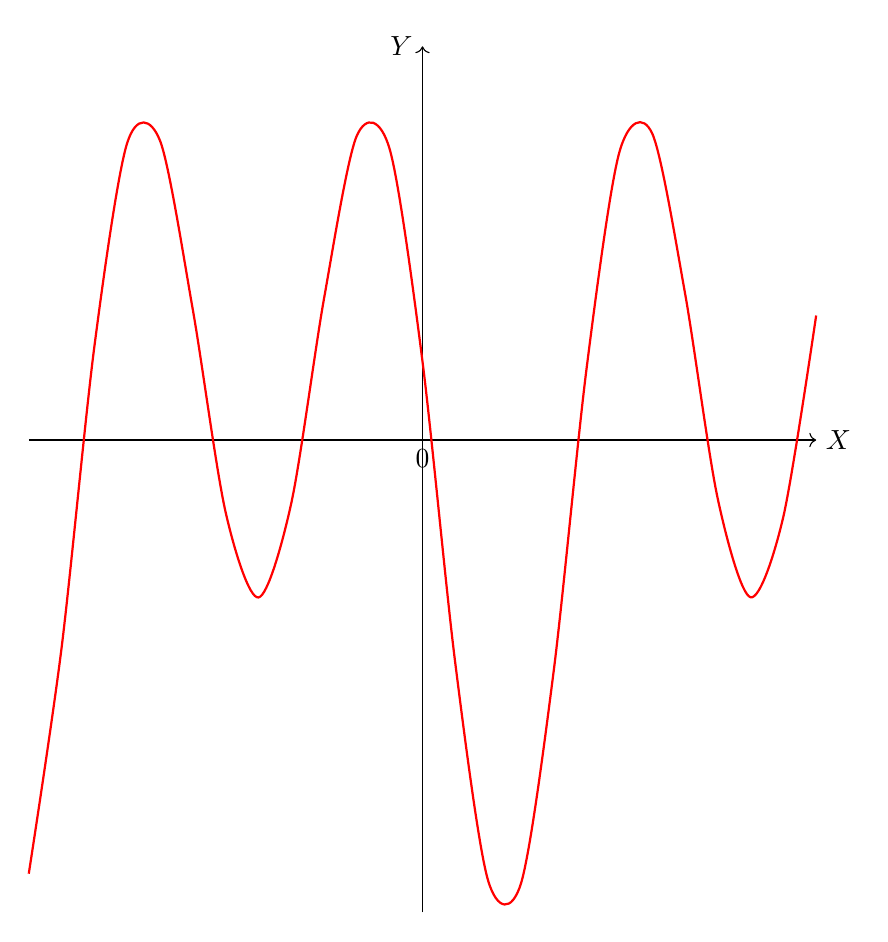
\begin{tikzpicture}[yscale=1,xscale=1]
%Построение осей
\draw[thin,->](-5,0)--(5,0) node [right] {$X$};
\draw[thin,->](0,-6)--(0,5) node [left] {$Y$};
%Построение графика производной на все участке
\draw [domain=-5:5, help lines,thick,smooth, red] plot (({\x},{4*cos((pi r+6*\x r)/3)-cos(\x r)-sqrt(3)*sin(\x r)});
\node [below] {$0$};
\end{tikzpicture}
\caption{Построение графика второй производной}
\label{fig:my_label}
\end{figure}
\clearpage

%%%%%%% 2 часть работы
\newpage
\section{Исследование кубического сплайна}
Для того чтобы потенциальная энергия изогнутой металлической линейки(сплайна) принимала минимальное значение,производная четвертого порядка должна быть равна нулю, следовательно можно представить сплайн полиномом третьей степени на каждом отрезке [$xi, x_{i+1}$]

\begin{figure}[!ht]
    \centering
\begin{tikzpicture}[yscale=1,xscale=3]
%Построение осей
\draw[thin,->](0,0)--(3.3,0) node [right] {$X$};
\draw[thin,->](0,0)--(0,4.6) node [left] {$Y$};
\node [below] {$0$};
%построение точек
\draw [ball color=black]
(0,4) circle (0.02) node [left] {$1$};
\draw [ball color=black]
(0.25,3.6) circle (0.02) node [above] {$2$};
\draw [ball color=black]
(1.25,4.575) circle (0.02) node [left] {$3$};
\draw [ball color=black]
(2.125,4.017) circle (0.02) node [left] {$4$};
\draw [ball color=black]
(3.25,3.83) circle (0.02) node [left] {$5$};
\end{tikzpicture}
\caption{Расположение точек на плоскости}
    \label{fig:my_label}
\end{figure}



Уравнение сплайна на 1 участке
\begin{equation}
y_1(x) =A_{10}+A_{11}x_1+A_{12}x^2_1+A_{13}x^3_1
\end{equation}
\begin{equation}
y_2(x) =A_{10}+A_{11}x_2+A_{12}x^2_2+A_{13}x^3_2
\end{equation}
\begin{equation}
y_2(x) =A_{20}+A_{21}x_2+A_{22}x^2_2+A_{23}x^3_2
\end{equation}
\begin{equation}
y_3(x) =A_{20}+A_{21}x_3+A_{22}x^2_3+A_{23}x^3_3
\end{equation}
\begin{equation}
y_3(x) =A_{30}+A_{31}x_3+A_{32}x^2_3+A_{33}x^3_3
\end{equation}
\begin{equation}
y_4(x) =A_{30}+A_{31}x_4+A_{32}x^2_4+A_{33}x^3_4
\end{equation}
\begin{equation}
y_4(x) =A_{40}+A_{41}x_4+A_{42}x^2_4+A_{43}x^3_4
\end{equation}
\begin{equation}
y_5(x) =A_{40}+A_{41}x_5+A_{42}x^2_5+A_{43}x^3_5
\end{equation}
Производные во внутренних точках

\begin{equation}
A_{11} + 2A_{12}x_2 + 3A_{13}x^2_2=A_{21} + 2A_{22}x_2 + 3A_{23}x^2_2
\end{equation}
\begin{equation}
A_{21} + 2A_{22}x_3 + 3A_{23}x^2_3= A_{31} + 2A_{32}x_2 + 3A_{33}x^2_3
\end{equation}
\begin{equation}
A_{31} + 2A_{32}x_4 + 3A_{33}x^2_4= A_{41} + 2A_{42}x_4 + 3A_{43}x^2_4
\end{equation}
Производные второго порядка в точках склейки
\begin{equation}
2A_{12} + 6A_{13}x_2=2A_{22} + 6A_{23}x_2
\end{equation}
\begin{equation}
2A_{22} + 6A_{23}x_3= 2A_{32} + 6A_{33}x_3
\end{equation}
\begin{equation}
2A_{32} + 6A_{33}x_4= 2A_{42} + 6A_{43}x_4
\end{equation}
Производные в крайних точках 1 и 5 равные нулю 
\begin{equation}
2A_{12} + 6A_{13}x_1=0
\end{equation}
\begin{equation}
2A_{42} + 6A_{43}x_5= 0
\end{equation}
В итоге составляется матрица вида

\resizebox{16cm}{!}{ %изменение размера матрицы
\begin{equation}
\left(
\begin{array}{cccccccccccccccc}
1 & x_1 & x_1^2 & x_1^3 & 0 & 0 & 0 & 0 & 0 & 0 & 0 & 0 & 0 & 0 & 0 & 0\\
1 & x_2 & x_2^2 & x_^3 & 0 & 0 & 0 & 0 & 0 & 0 & 0 & 0 & 0 & 0 & 0 & 0\\
0 & 1 & 2x_2 & 3x_2^2 & 0 & -1 & -2x_2 & -3x_3^2 & 0 & 0 & 0 & 0 & 0 & 0 & 0 & 0\\
0 & 0 & 2 & 6x_2 & 0 & 0 & -2 & -6x_2 & 0 & 0 & 0 & 0 & 0 & 0 & 0 & 0\\
0 & 0 & 0 & 0 & 1 & x_2 & x_2^2 & x_2^3 & 0 & 0 & 0 & 0 & 0 & 0 & 0 & 0\\
0 & 0 & 0 & 0 & 1 & x_3 & x_3^2 & x_3^3 & 0 & 0 & 0 & 0 & 0 & 0 & 0 & 0\\
0 & 0 & 0 & 0 & 0 & 1 & 2x_3 & 3x_3^2 & 0 & -1 & -2x_3 & -3x_3^2 & 0 & 0 & 0 & 0\\
0 & 0 & 0 & 0 & 0 & 0 & 2 & 6x_3 & 0 & 0 & -2x_3 & -6x_3 & 0 & 0 & 0 & 0\\
0 & 0 & 0 & 0 & 0 & 0 & 0 & 0 & 1 & x_3 & x_3^2 & x_3^3 & 0 & 0 & 0 & 0\\
0 & 0 & 0 & 0 & 0 & 0 & 0 & 0 & 1 & x_4 & x_4^2 & x_4^3 & 0 & 0 & 0 & 0\\
0 & 0 & 0 & 0 & 0 & 0 & 0 & 0 & 0 & 1 & 2x_4 & 3x_4^2 & 0 & -1 & -2x_4 & -3x_4^2\\
0 & 0 & 0 & 0 & 0 & 0 & 0 & 0 & 0 & 0 & 2 & 6x_4 & 0 & 0 & -2 & -6x_4\\
0 & 0 & 0 & 0 & 0 & 0 & 0 & 0 & 0 & 0 & 0 & 0 & 1 & x_4 & x_4^2 & x_4^3\\
0 & 0 & 0 & 0 & 0 & 0 & 0 & 0 & 0 & 0 & 0 & 0 & 1 & x_5 & x_5^2 & x_4^3\\
0 & 0 & 2 & 6x_1 & 0 & 0 & 0 & 0 & 0 & 0 & 0 & 0 & 0 & 0 & 0 & 0\\
0 & 0 & 0 & 0 & 0 & 0 & 0 & 0 & 0 & 0 & 0 & 0 & 0 & 0 & 2 & 6x_4

\end{array}
\right)*


\left(
\begin{array}{c}
A_{10} \\
A_{11} \\
A_{12} \\
A_{13} \\
A_{20} \\
A_{21} \\
A_{22} \\
A_{23} \\
A_{30} \\
A_{31} \\
A_{32} \\
A_{33} \\
A_{40} \\
A_{41} \\
A_{42} \\
A_{43} \\
\end{array}
\right)
=
\left(
\begin{array}{c}
y_1 \\
y_2 \\
0 \\
0 \\
y_2 \\
y_3 \\
0 \\
0 \\
y_3 \\
y_4 \\
0 \\
0 \\
y_4 \\
y_5 \\
0 \\
0 \\
\end{array}
\right)
\end{equation}
}

Решение системы уравнений
\left(
\begin{array}{c}
A_{10} \\
A_{11} \\
A_{12} \\
A_{13} \\
A_{20} \\
A_{21} \\
A_{22} \\
A_{23} \\
A_{30} \\
A_{31} \\
A_{32} \\
A_{33} \\
A_{40} \\
A_{41} \\
A_{42} \\
A_{43} \\
\end{array}
\right)=
\left(
\begin{array}{r}
4 \\
-1,956 \\
0 \\
5,965 \\
4,127 \\
-3,475 \\
6,077 \\
-2,408 \\
-0,2 \\
8,303 \\
-4,461 \\
0,7 \\
-1,165 \\
9,67 \\
-5,104 \\
0,801 \\
\end{array}
\right)

Окончательно, уравнение для сплайна получается в виде
\begin{equation}
F(x)=\left\{
\begin{array}{l}
    F_1(x)=5.965x^3-1.956x+4\\
    F_2(x)=-2.408x^3+6.077x^2-3.475x+4.127\\
    F_3(x)=0.7x^3-4.46x^2+8.303x-0.2\\
    F_4(x)=0.801x^3-5.104x^2+9.67x-1.165\\
\end{array}
\right.
\end{equation}
График функции F(x) представлен на рисунке 7
%Построение сплайна
\begin{figure}[!ht]
    \centering
\begin{tikzpicture}[yscale=3,xscale=3]
%Построение осей
\draw[thin,->](0,3.4)--(4,3.4) node [right] {$X$};
\draw[thin,->](0,3.4)--(0,5) node [left] {$Y$};
\draw (0,3.2) node {$0$};


%Построение графика сплайна
\draw [domain=0:0.25,thick,smooth, red] plot ({\x},{5.965*(\x^3)-1.956*(\x)+4});%1 график
\draw [domain=0.25:1.25,thick,dashed, black] plot ({\x},{-2.408*(\x^3)+6.077*(\x^2)-3.475*(\x)+4.127});%2 график
\draw [domain=1.25:2.125,thick,smooth, yellow] plot ({\x},{0.7*(\x^3)-4.46*(\x^2)+8.303*(\x)-0.2});%3 график
\draw [domain=2.125:3.25,thick,dotted, brown] plot ({\x},{0.801*(\x^3)-5.104*(\x^2)+9.67*(\x)-1.165});%4 график

\end{tikzpicture} 
    \caption{Построение сплайна}
    \label{fig:my_label}
\end{figure}
\clearpage
%Оценка погрешности
\subsection{Оценки погрешности интерполяции эрмитовыми кубическими сплайнами}
Согласно задания необходимо вычислить значение функции в точке х1=1,2 на 4 участке и вычислить погрешность в точке х0=2,2
\begin{equation}
\mid S^{(r)}_3(x) - f^{(r)}(x) \mid \leqslant \mathcal{R}_r, r=0,1,2,3
\end{equation}

Если функция достаточно гладкая, то
\begin{equation}
\mid S^{(r)}_3(x) - f^{(r)}(x) \mid \leqslant \frac{1}{384} \bar{h}^4 \mid f^{IV}(x)\mid 
\end{equation}

где,
\begin{equation}
\bar{h} = \left| x_{\tiny{\begin{array}{l}\textcyrillic{точка, в которой}\\ \textcyrillic{вычисляется}\\ \textcyrillic{погрешность}\end{array}}} -
x_{\scriptstyle\tiny{{\textcyrillic{ближайшее }i}}}\right|\\
\end{equation}

Откуда знчение функции $F_4(x)=0.801x^3-5.104x^2+9.67x-1.165$ равно

F_4(1,2)=4.473368

Погрешность равна
\begin{equation}
\mid S^{(r)}_3(x) - f^{(r)}(x) \mid \leqslant \frac{1}{384} \bar{|2.2-2.12|}^4*4.473368=0.0000004
\end{equation} 
\newpage
% 3 задача
Задание 3
Решить задачу оптимального распределения неоднородных ресурсов. На предприятии постоянно возникают задачи определения
оптимального плана производства продукции при наличии конкретных ресурсов (сырья, полуфабрикатов, оборудования, финансов, рабочей силы и др.) или проблемы оптимизации распределения неоднородных ресурсов на производстве. Рассмотрим несколько возможных примеров постановки таких задач.В таблице приведены исходные данные для расчета.

Таблица 1 Исходные данные для расчета

\begin{tabular}{|c|r|r|r|r|r|}
\hline
используемые ресурсы & И_1 & И_2 & И_3 & И_4 & наличие ресурсов \\
\hline
трудовые & 3 & 5 & 5 & 3 & 11 \\
\hline
материальные & 4 & 5 & 8 & 5 & 8 \\
\hline
финансовые & 5 & 6 & 4 & 8 & 26 \\
\hline
прибыль & 40 & 50 & 25 & 25 &  \\
\hline
\end{tabular}

Для расчета будет использован математический пакет Scilab. Ниже описаны основные переменные необходимые для расчета.
Для решения задачи предназначена функция linpro. Синтаксис записи приведен ниже:
\begin{equation}
$$[x,larg,f]=linpro(p,C,b[ci,cs])$$
\end{equation}
Где р-вектор-столбец коэффициентов при неизвестных целевой функции
С-матрица при неизвестных из левой части системы ограничений
b-вектор-столбец содержит свободные члены системы ограничений
ci-вектор-столбец содержит нижнюю границу переменных
cs-вектор-столбец содержит верхнюю границу переменных

Система ограничений
\begin{equation}
\left\{
\begin{array}{l}
    3x_1+5x_2+5x_3+3x_4 \leq 11\\
    4x_1+5x_2+8x_3+5x_4 \leq 8\\
    5x_1+6x_2+4x_3+4x_4 \leq 26\\
\end{array}
\right.
\end{equation}
Целевая функция 
\begin{equation}
F_{max}=40x_1+50x_2+25x_3+25x_4
\end{equation}

\begin{equation}
C = \begin{pmatrix}
3 & 5 & 5 & 3 \\
4 & 5 & 8 & 5 \\         
5 & 6 & 4 & 4 \\
\end{pmatrix}
\end{equation}
\begin{equation}
b = \begin{pmatrix}
11  \\
8  \\         
26  \\
\end{pmatrix}
\end{equation}
\begin{equation}
p = \begin{pmatrix}
40 \\
50 \\         
25 \\
25 \\
\end{pmatrix}
\end{equation}

В итоге были рассчитаны основные параметры при которых возможна максимальная прибыль:

Целевая функция $$F_{max}=80$$

$$larg=(0;0;55;25;0;10;0)$$

$$x=(0;1.6;0;0)$$

Из чего следует максимальная прибыль будет при производстве 1,6 изделия И_2
\clearpage
\newpage
\section{Заключение}
В ходе курсовой работы были выполнены ряд исселований,касающихся поведения функции на ограниченном участке, построены ее графики функции включая производные. Определены характерные точки.
При использовании математических пакетов было решено уравнение и найдены его корни.
В последней части работы были расчитаны коэффциенты кубического сплайна и составлены зависимости, которые были отражены непосредственно кривой на плоскости координат Х и У. Была расчитана погрешность, с точностью до 8 знака.
В заключительной части курсовой работы была решена задача, на оптимальные параметры.
\clearpage
\section{Список литературы}
[1] Ю.С. Завьялов. Методы сплайн-функций. М.Наука, 1980.

[2] Калиткин. Численные методы. М.,Мир, 1980.

[3] Разделённая разность. 2015. url:https://ru.wikipedia.org/wiki/%D0%A0%D0%B0%D0%B7%D0%B4%D0%B5%D0%BB%D1%91%D0%BD%D0%BD%D0%%D1%8F_%D1%80%D0%B0%D0%B7%D0%BD%D0%BE%D1%81%D1%82%D1%8C.

[4] Решение задач оптимизации средствами Scilab и Excel : Методические указания к лабораторной работе по дисциплине «Математическая экономика» / Уфимск. гос. авиац. техн. ун-т; Сост.: Л.М. Бакусов, О.В. Кондратьева - Уфа, 2011. - 33 с.

[5] Андриевский А.Б., Андриевский Б.Р., Капитонов А.А., Фрадков А.Л. РЕШЕНИЕ ИНЖЕНЕРНЫХ ЗАДАЧ В SCILAB - Санкт-Петербург: НИУ ИТМО, 2013. - 97 с. - экз.

\end{document}